
\item Sand is pouring from a pipe at the rate of $ 15 cm^3/minute$. The falling sand forms a cone on the ground such that the height of the cone is always one- third of the radius of the base. How fast is the height of the sand cone increasing at the instant when the height is $4cm$	 


\item A rectangular visiting card is to contain $24 sq.cm.$ of printed matter. The margins at the top and bottom of the card are to be $1 cm$ and the margins on the left and right are to be cm as shown below:

%\newpage
\begin{figure}[h!]
\centering
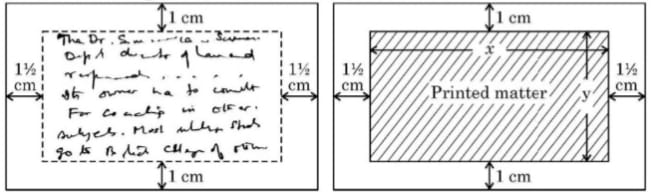
\includegraphics[width=0.8\textwidth]{figs/fig2.jpg}
\label{fig:image2}
\end{figure}

On the basis of the above information, answer the following questions:
\begin{enumerate}
	\item[(i)] Write the expression for the area of the visiting card in terms of x.

	\item[(ii)] Obtain the dimensions of the card of minimum area.



\end{enumerate}


\end{enumerate}
